\chapter{Indledning}
Aalborg Kommune er med et indbyggertal på over 205.000 og et areal på cirka  1.140 $km^2$, landets tredjestørste kommune målt på indbyggertal og landets anden største kommune målt på areal \citep{indbyggertal}. Det område, som Kommunen dækker, er vist på Figur \ref{fig:aalborgkommune}. 
\newline \indent{     }  Aalborg er en tidligere industriby og førhen var industriområderne placeret i Aalborg Centrum. Nye planer for Aalborg har ført denne industri ud i nogle yderpunkter af Aalborg by. Derfor har kommunen nye visioner om at flytte kultur, studieliv og turisme ind, hvor der før var industri. Kommunens visioner omkring byens udvikling fremgår af Kommuneplanen, hvor det primære fokus i denne rapport vil være et område gennem Aalborg, der er tiltænkt mest vækst, dette betegnes som Vækstaksen (se Figur \ref{fig:vaekstakse}).
\newline \indent{     }  Indenfor de seneste 5-10 år har Aalborgs centrale havnefront gennemgået en stor udvikling. Denne er stadig i gang, hvilket ses ved, at der kommer flere boligbyggerier til havnen, som Strøybergs Palæ er en del af. 
\newline \indent{     }  Det har siden år 2010 været på tale, at lave en tilbygning til den bevaringsværdige bygning, Strøybergs Palæ. Bygningen er fra år 1908 \citep{byggesagen}, beliggende centralt i Aalborg ved Slotspladsen, der er en cirka 200 meter vejstrækning og plads ved Aalborgs centrale havnefront, samt i nærheden af museet Utzon Centret og overfor shoppingcentret Friis. Figur \ref{fig:aalborg} viser Strøybergs Palæs beliggenhed. 
\newline \indent{     }  Når der skal anlægges nye arealer, bygninger, veje osv., skal det opføres i henhold til en lokalplan, der dækker et mindre område inden for kommunen, og har til formål at styre udviklingen indenfor dette område ved hjælp af fastlagte regler og målsætninger. Den gældende lokalplan for området ved Strøybergs Palæ er lokalplan 1-1-107. 

\begin{figure}[htbp] \centering
	\begin{minipage}[b]{0.48\textwidth}\centering
		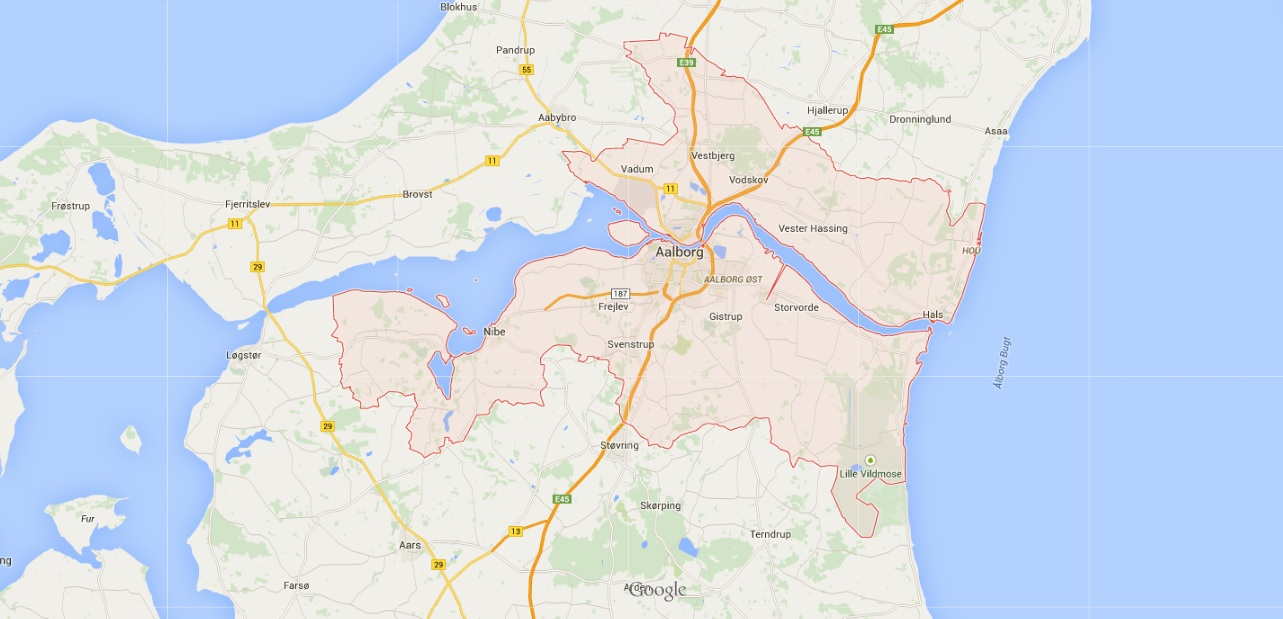
\includegraphics[width=0.6\textwidth]{billeder/aalborgkommune.png}
		\caption{Aalborg Kommune}
		\label{fig:aalborgkommune}
	\end{minipage}\hfill
	\begin{minipage}[b]{0.48\textwidth}\centering
		\centering
		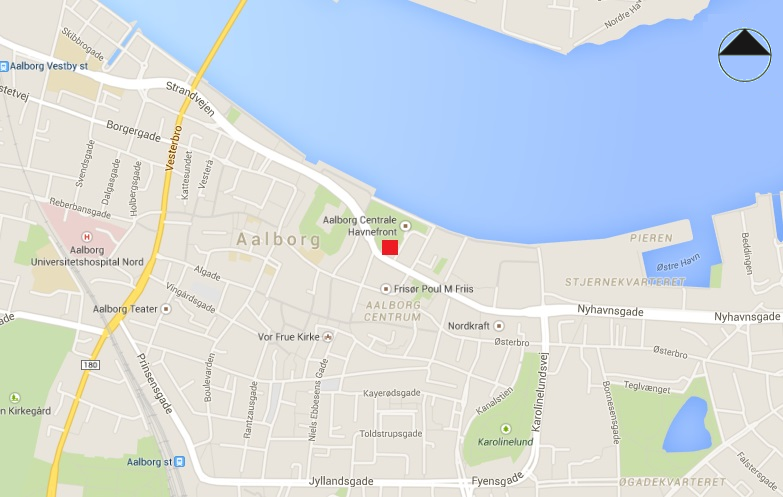
\includegraphics[width=0.6\textwidth]{billeder/aalborg.png}
		\caption{Strøybergs Palæs beliggenhed}
		\label{fig:aalborg}
	\end{minipage}
\end{figure}